\chapter{Method}
\label{chap:method}

In this chapter I first describe techniques that lie in core of the proposed solution.
They then followed by a detailed explanation of the proposed solution.
Finally I give the implementation details and settings.

\section{Neural Radiance Fields}

The Neural Radiance Fields approach (\cite{mildenhall2020nerf}) lies directly in the heart of the proposed solutions.
The continuous 5D function 

\begin{equation}
    \label{eq:nerf_function}
    F : (p,v) \xrightarrow{} (c, \sigma)
\end{equation}

is required to be achieved in order to solve the novel view synthesis problem.
Given the spatial location $p \in \mathbb{R}^3$ and the 2D viewing direction $(\theta, \phi)$ (or its equivalent 3D Cartesian representation $v \in \mathbb{R}^3$),
one has to obtain the RGB color value $c$ and the volume density $\sigma$ at this exact point $p$ under the viewing direction $v$.
To obtain the image of the scene, one can take a pin-hole camera at position $p_0$ and cast rays to the scene: $p(z) = p_0 + z\cdot v$.
The final visible color value $C(p,v)$ can then be evaluated using volume rendering approach \cite{niemeyer2020differentiable, Novak18volumeSTAR} along the ray $p$:
\begin{equation}
    C(p,v) = \int_{0}^{\infty} \omega(p(z)) \cdot c(p(z),v) dz,
    \label{eq:rendering_equation}
\end{equation}
$\omega(p(z))$ is a probability weight function
\begin{equation}
    \omega(p(z)) = \tau_c(p(z)) \sigma(p(z)),
\end{equation}
where $\tau_c(p(z)) = e^{\int_0^z \sigma(p(s)) ds}$ denotes the accumulated transmittance along the ray up to the point $p(z)$, $\sigma(p(z))$ is the volume density at point $p(z)$ and the probability property is held: $\int_0^\infty \omega(p(z))dz = 1$

\begin{figure}[!htb]
    \centering
    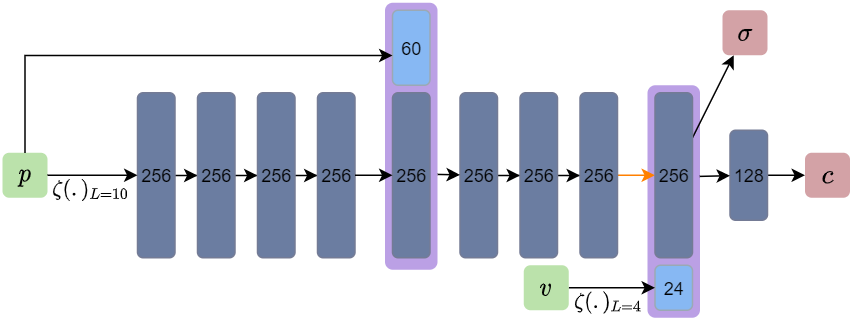
\includegraphics[width=0.9\textwidth]{figures/mlp_nerf.png}
    \caption{MLP used in NeRF \cite{mildenhall2020nerf} Dark blue boxes represent hidden layers. Black arrows indicate FC-layers with sigmoid activation, orange arrows - FC-layers without activation. Green boxes are inputs: $p$ is a 3D sample point, $v$ is a 3D vector of viewing direction. Red boxes are the outputs: $\sigma$ is 1D volume density, $c$ is a 3D color value. $\zeta(.)$ stands for positional encoding function that maps inputs into higher dimensional space $\mathbb{R}^{2L}$ (more in \Cref{subsec:pos_enc}}
    \label{fig:mlp_nerf}
\end{figure}

\cite{mildenhall2020nerf} propose to use a Multi-Layer Perceptron (MLP) as a representation
of an implicit function $F = F_\Theta$ with parameters $\Theta$.
The scheme structure of original NeRF's MLP is outlined in \Cref{fig:mlp_nerf}.
The position $p(z)$ is first encoded using position encoding function $\zeta(\cdot)$ (positional encoding is described in section \ref{subsec:pos_enc}) and then is processed with 8 fully-connected neural layers with ReLU activations.
The resulting feature vector is then concatenated with positionally encoded vector direction $v$
before the volume density $\sigma(p(z))$ and the color value $c(p(z), v)$ is outputed.
The important concept here is that $\sigma$ only depends on point $p(z)$
whilst the color value $c$ is view dependant as well.
This setting is required to encourage the MLP to be multi-view consistent.

In order to perform the volume rendering, the continuous integral from equation \Cref{eq:rendering_equation} has to be solved.
One can estimate this integral using a discrete set of densely sampled points as proposed by \cite{mildenhall2020nerf}.
Separating each ray into $N$ bins and drawing random samples from each bin
makes the representation able to learn continuous function
while only using finite number of samples.
The estimate for the integral $C(p, v)$ will have a form (\cite{mildenhall2020nerf, max1995optical}):
\begin{equation}
    \label{eq:integral_estimation}
    C(p, v) \approx \sum_{i=1}^{N} \tau_c(p_i) (1 - \exp (-\sigma(p_i) \delta_i)) c(p_i, v),
\end{equation}
where $p_i = p(z_i)$ for brevity, $\tau_c(p_i) = \exp (-\sum_{j=0}^i \sigma(p_j) \delta_j )$ is the accumulated transmittance and $\delta_i = z_{i+1} - z_i$ is the distance between adjacent sample points.

\subsection{Positional encoding}
\label{subsec:pos_enc}

Neural networks are known as a highly representative class of functions (\cite{hornik1989multilayer}).
However, recent works (\cite{rahaman2019spectral, tancik2020fourfeat}) demonstrate the tendency of
biasing towards low frequency functions during training of deep neural networks.
The results can be smoothed and blurry as frequency-dependant learning speed
is much slower for high-frequency parts of the scene.
\cite{rahaman2019spectral} show that one can highly improve the quality of the MLP outputs
by using an embedding, which maps inputs to a higher dimensional space before passing them to the MLP.

The positional encoding function $\zeta(p) : \mathbb{R} \xrightarrow{} \mathbb{R}^{2L}$ as proposed by \cite{mildenhall2020nerf, vaswani2017attention} is represented by Fourier series in the following form:
\begin{equation}
    \label{eq:positional_encoding}
    \zeta(x) = (\sin(2^0\pi x), \cos(2^0\pi x), ..., \sin(2^{L-1}\pi x), \cos(2^{L-1}\pi x))
\end{equation}
The 3D Cartesian coordinates of $p$ and $v$ are then separately transformed using $\zeta(\cdot)$ and concatenated.


\subsection{Hierarchical sampling}
\label{subsec:hierarchy_sampling}

The proposed approach is ineffective in a way that it tends to generate a lot of unimportant samples
that lie on a free space and do not contribute much.
To solve that authors propose the hierarchical volume sampling algorithm (similar to \cite{levoy1990efficient}),
when another "coarse" neural network is used in order to roughly estimate volume densities along the ray.
This insight is then used to perform a more informed sampling of main ("fine") network.
The "coarse" network is being optimized along with the main network, which can be considered as an overhead.
However, taking into account the increase of training convergence the overall training gets more efficient.


\subsection{Optimization}

The fully-differentiable formulation of the problem makes it possible
to optimize network parameters $\Theta$ without any 3D supervision.
This is done using the back-propagation approach from the differences
between rendered predictions and ground truth images.
This task therefore is reduced to the minimization problem of the loss function.
The original method by \cite{mildenhall2020nerf} for loss function uses the following formulation:
\begin{equation}
    \label{eq:loss_func}
    \mathcal{L} = \sum_{(p_0, v) \in \mathcal{B}} \norm{ C_c(p, v) - C^*(p, v) }^2_2 + \norm{ C_f(p, v) - C^*(p, v) }^2_2,
\end{equation}
where $\mathcal{B}$ is the set of sampled rays in each batch,
$C^*$ is the target color value of the view ray $v$ and
$C_c(p, v)$, $C_f(p, v)$ - are the predicted colors for the view ray $v$ of the coarse and fine networks respectively.

Another regularization term can be added to this loss function as proposed by \cite{Lombardi_2019}.
The beta-distribution regularizer $\Omega(\cdot)$
forces the ray transmittance from the fine network $\tau_c$ to be close to $0$ or $1$:
\begin{equation}
    \label{eq:beta_regularizer}
    \Omega(\tau_c(p_i)) = \log(\tau_c(p_i)) + \log(1 - \tau_c(p_i))
\end{equation}
This helps the network to better handle background colors and get cleaner render after all.
This regularization term is used in NSVF work (\cite{liu2021neural})
that is described in \Cref{subsec:NSVF}
and NRF work (\cite{bi2020neural}) that is described in \Cref{subsec:NRF}



\subsection{Sparse Voxels Octree}
\label{subsec:NSVF}
The described approach is already able to represent scenes with high accuracy.
However, the very inefficient way of sampling points along rays
makes the training very slow and tough,
since the model has to be repeatedly evaluated on unimportant samples
of free space or occluded regions that do not make a worthwhile contribution to the finally rendered color value.
The \textit{hierarchical sampling} strategy alleviates the problem,
but does not solve it completely.
The method in its formulation therefore is still barely practical.


\cite{liu2021neural} propose another framework
that is able to increase the efficiency of this method
and make the training time by up to an order of magnitude faster.
The main contribution is the usage of sparse voxel octrees (\cite{laine2011EfficientSV}) to divide space into voxels
that are efficiently used for training MLPs with shared parameters.

This approach requires a slight elaboration on the problem formulation.
Let the whole scene be fully contained in a set of $K$ sparse voxels: $\mathbb{V} = \{V_k\}_{k=1}^K$.
The scene can then be represented as a set of voxel-bounded implicit functions
\begin{equation}
    F(p, v) = F_\Theta^i(g_i(p), \zeta(v)), \forall p \in V_i,
\end{equation}
where each function $F_\Theta^i$ is modelled with an MLP with shared parameters $\Theta$:
\begin{equation}
    F_\Theta^i: (g_i(p), \zeta(v)) \xrightarrow{} (c, \sigma), \forall p \in V_i
\end{equation}
Here $g_i(p)$ is the representation of $p$ that is defined as:
\begin{equation}
    g_i(p) = \zeta ( \chi ( \{\Tilde{g_i}(p_j^*)\}_{j=1}^8 ) ),
\end{equation}
where $\{p_j^*\}_{j=1}^8, p_j^* \in \mathbb{R}^3$ is the set of eight vertices of voxel $V_i$,
$\Tilde{g_i} \in \mathbb{R}^d$ represent the feature vectors that are stored for each vertex of voxel $V_i$,
$\chi(\cdot)$ stands for trilinear interpolation,
and $\zeta(\cdot)$ is a post-processing function,
which corresponds to positional encoding function explained in \ref{subsec:pos_enc}.


\begin{figure}[!htb]
    \centering
    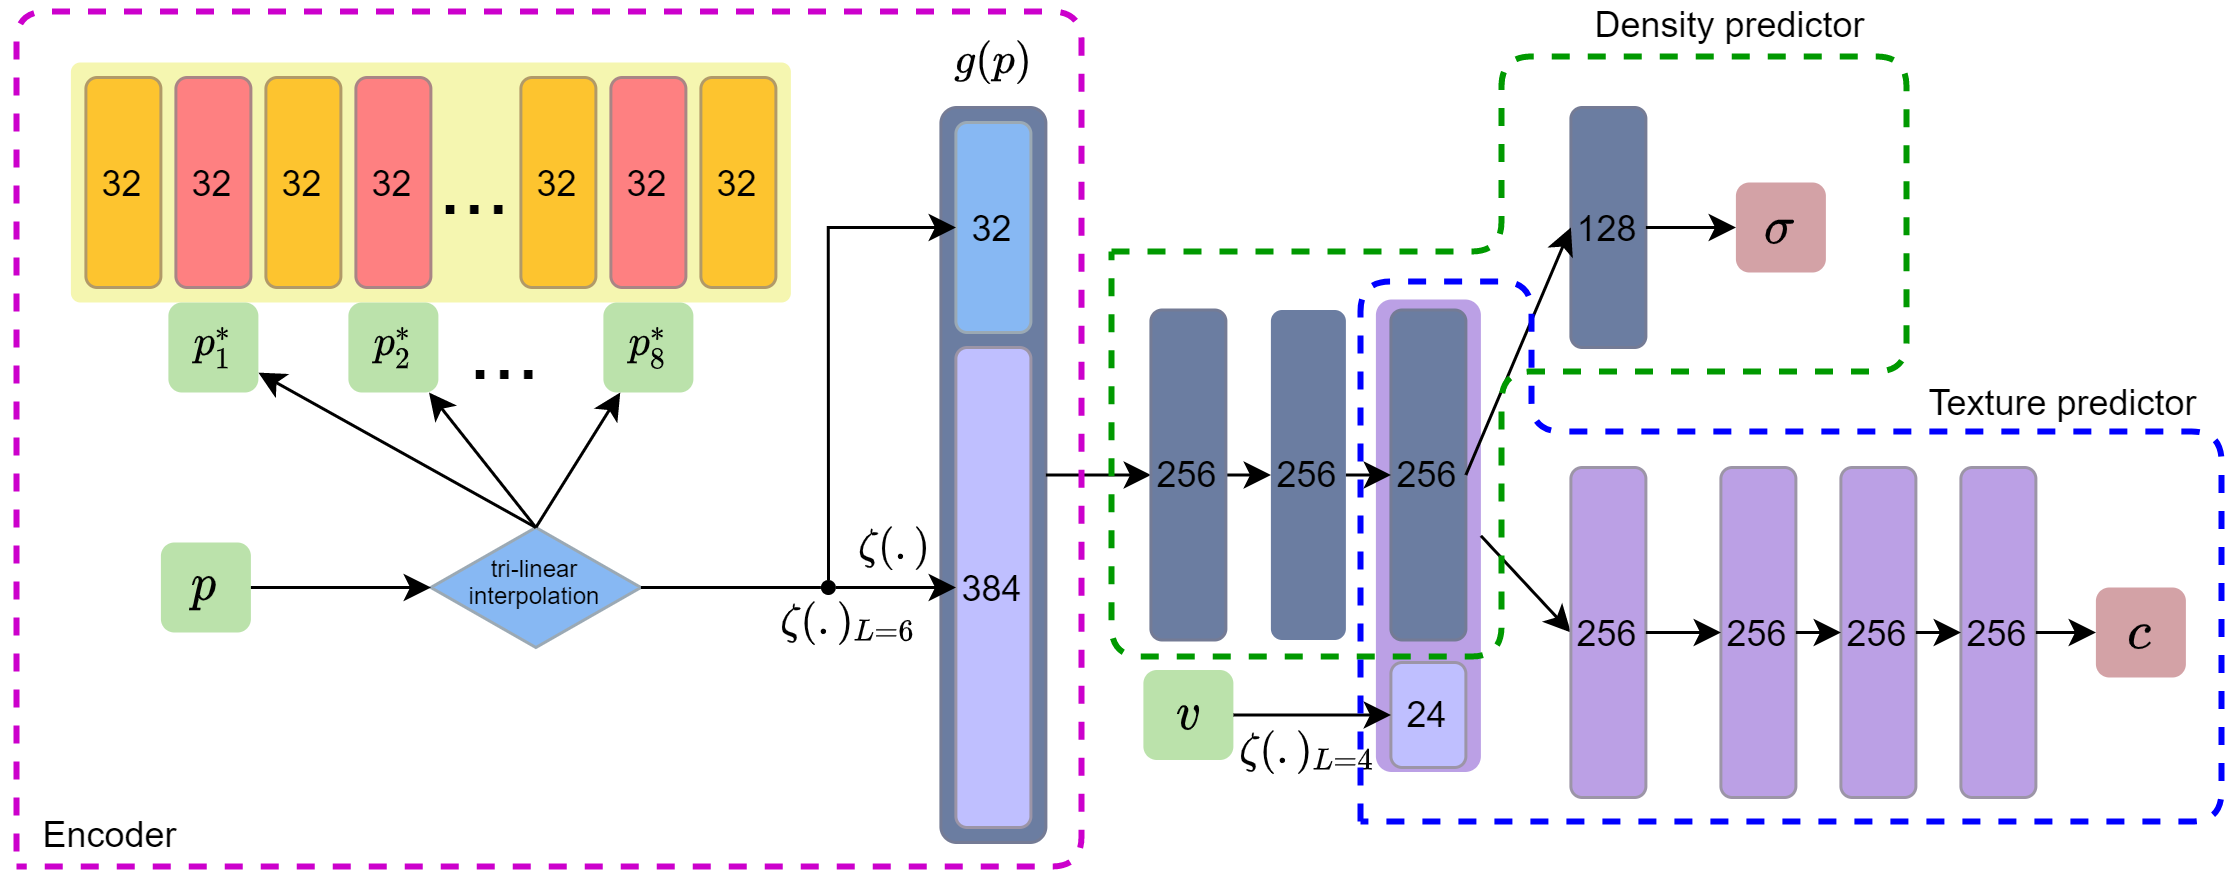
\includegraphics[width=0.9\textwidth]{figures/vanilla_nsvf.png}
    \caption{Network structure of the NSVF approach
(the figure is adapted from \cite{liu2021neural}).
Same notation as for \Cref{fig:mlp_nerf} is used.
Dotted lines denote semantic parts of the presented structure:
pink, green and blue dotted lines stand for encoder, density predictor and texture predictor respectively.
\textit{Trilinear interpolation} block denotes interpolation of the sample point $p$ between voxel embeddings.}
    \label{fig:nsvf_structure}
\end{figure}

The proposed network structure is outlined in \Cref{fig:nsvf_structure}.
The encoder part that is denoted with pink dotted line
consists of only one layer comparing to the original NRF network
where the encoder part consists of 5 deep layers.
The density predictor (green dotted line) remains the same.
The texture predictor (blue dotted line) is deeper comparing to the NeRF model.
The overall model structure is slightly shallower comparing to the original NeRF network,
which is still sufficient due to the distributed way of storing voxel embeddings in the voxel vertices.
Without voxel embeddings the model contains approximately 0.5M learnable parameters,
which is lower than in the original NeRF model.

The volumetric rendering itself does not undergo any significant changes
except for some additional steps that have to be performed.
The sampling of the ray is only performed on the intervals of intersection with voxels $V_i$.
This allows to reject a descent amount of unimportant samples.
A very efficient Axis Aligned Bounding Box (AABB) ray intersection algorithm (\cite{haines1989essential}) is applied here
to extract the above mentioned intervals.
Another step is \textit{early termination}, which reduces the number of samples that have to be processed.
Since solid surfaces does not imply color values being dispersed along the ray,
the sample points that are behind the surface would be needless.
The technique here is to straight forwardly stop evaluating points,
that have an accumulated transmittance lower than some threshold.

\subsection{Voxels pruning and refinement}
\label{subsec:pruning}

The training on the scene begins with the octree,
which consists of $N=N^3_0$ voxels that fit in bounding box of the whole scene
and cover all parts of the scene.
One can get rid of non-essential voxels by performing a \textit{self-pruning} procedure.
This technique leverages the property of neural radiance fields
to extract some coarse scene geometry during early training iterations.
The decision if voxel is going to be pruned is made by uniformly sampling $G$ points inside the voxel
and comparing the minimum transmittance value with some threshold value $\gamma$ or more formally when:
\begin{equation}
    \underset{j=1 \dots G}{min} {\exp (- \sigma (g_i(p_j)))} > \gamma, p_j \in V_i, V_i \in \mathbb{V},
\end{equation}
where $\sigma (g_i(p_j))$ is the model prediction for $\sigma$ when processing $g_i(p_j)$.
The pruning procedure has to be performed regularly as the accuracy of the model increases as it gets more and more trained,
which means that more voxels can be pruned and therefore rejected from processing.

As model learns more detailed representation of the scene it becomes necessary to refine voxel structure.
During the refinement procedure each voxel is being subdivided into $2^3$ subvoxels by halving the voxel size.
Ray sampling steps are also being halved at this point in order to correspond new voxel size value.
The feature representation vectors $\Tilde{g_i}$ of the new vertices are initialized similarly to calculating $G_i(p)$,
namely using trilinear interpolation function $\chi(\cdot)$.
This scheme allows to achieve more detailed scene representation
and also increases the model capacity.



\subsection{Neural Reflectance Fields}
\label{subsec:NRF}

Although the neural radiance fields approach is able to produce realistic renderings under novel view conditions,
one of main limitations of this method is the inability to handle any kind of visual effects related to dynamic light conditions.
The core assumption of these approaches is a static illumination,
which is implicitly presented in the color values of the rendered images.
This in turn does not allow to change illumination on the rendering phase.

\cite{bi2020neural} propose the framework for eliminating this exact limitation.
Authors introduce neural reflectance field (NRF), which is the neural scene representation
that in addition to scene geometry also encodes normal and reflectance properties of the scene.
This approach allows to evaluate an explicit reflectance model at the selected point after all.
Although \cite{bi2020neural} focus on the microfacet bidirectional reflectance distribution function (BRDF) (\cite{walter2007microfacet}),
any other reflectance model can be used within this method as well
(i.e. authors also show some results of furry objects using hair reflectance model \cite{kajiya1989fur}).

This method uses the same rendering framework as proposed by \cite{mildenhall2020nerf}.
Assuming that the volume containing the scene to be only scattering volume (i.e. there are no emission or absorption processes),
the corresponding rendering equation \Cref{eq:rendering_equation} (\cite{Novak18volumeSTAR}) looks similarly
except for operating with radiance values $L$ instead of color values $c$:
\begin{equation}
    L(p, v) = \int_0^\infty \omega(p(z)) \cdot L_s(p(z), v) dz = \int_0^\infty \tau_c(p(z)) \sigma(p(z)) \cdot L_s(p(z), v)dz,
\end{equation}
where $L_s(p(z), v)$ denotes the scattered light at point $p(z)$ along direction $v$.

In general case $L_s$ is calculated by integrating incident radiance along the whole unit sphere $\mathbb{S}$:
\begin{equation}
    \label{eq:radiance_Li}
    L_s(p, v) = \int_\mathbb{S} f_p(p, v, l) L_i(p, l)dl,
\end{equation}
where $l$ is the 3D Cartesian representation of directions of the incident radiance $L_i(p, l)$.
$f_p(p, v, l)$ is the phase function, which controls
how the light that comes from $l$ scatters at point $p$ if viewing from $v$.

\cite{bi2020neural} only assume single light source setting
and the reflectance function as the phase function,
which allows to simplify \Cref{eq:radiance_Li}:
\begin{equation}
    L_s(p, v) = f_r(p, v, l, n(p), R(p)) L_i(p, l),
\end{equation}
where $f_r$ denotes a differentiable reflectance function
with parameters $R$.
Normal vector $n$ is also required for evaluation of reflectance model $f_r$.
$L_i(p, l)$ is the radiance that arrives from direction $l$ and can be calculated using light intensity $L_l(p)$
and the transmittance value $\tau_l(p, l)$,
which indicates the loss of light from the light source to the sample point $p$ along light ray $l$, as follows:
$L_i(p, l) = \tau_l(p, l) L_l(p, l)$.
The light attenuation coefficient $f_{att} = \frac{1}{k_c + k_l d + k_q d^2}$ \cite{madams2011attenuation, madams2011improved} is considered inside the $L_l$ term:
$L_l(p, l) = f_{att} \cdot I$,
where $k_c$, $k_l$ and $k_q$ are attenuation factors,
$I$ is the point light intensity.
% where $d$ is distance from sample point $p$ to the light source
% and $r$ is the light's radius (assuming light source to be an emissive sphere with radius $r$) and 
In my experiments the attenuation coefficients $k_c = k_l = 0$ and $k_q = 1$ were used,
so the attenuation coefficient is inverse proportional to squared distance between light sample point and light source:
$f_{att} = \frac{1}{d^2}$

Combining these equations together and applying the same technique for numerical integral estimation
as used by \cite{mildenhall2020nerf} and \cite{liu2021neural} gives the following formulation of \Cref{eq:integral_estimation} for NRF:
\begin{equation}
    \label{eq:integral_estimation_nrf}
    L(p, v, l) \approx \sum_{i=1}^N \tau_l(p_i, l) L_l(p_i, l) f_r(p_i, v, l, n(p_i), R(p_i)) \tau_c(p_i) (1 - \exp (-\sigma(p_i)\delta_i))
\end{equation}
Here $\tau_l$ plays the same role for light ray $l$
as $\tau_c$ operates for view ray $v$.
It is evaluated similarly along the light ray $l$:
$\tau_l(p'_i, l) = \exp (-\sum_{j=1}^M \sigma(p'_j) \delta'_j)$,
where $p'(z') = p'_0 + z' \cdot l$ are sample points that are additionaly sampled along the light ray $l$ and $\delta'_j = z'_{j=1} - z'_j$.


\begin{figure}[!htb]
    \centering
    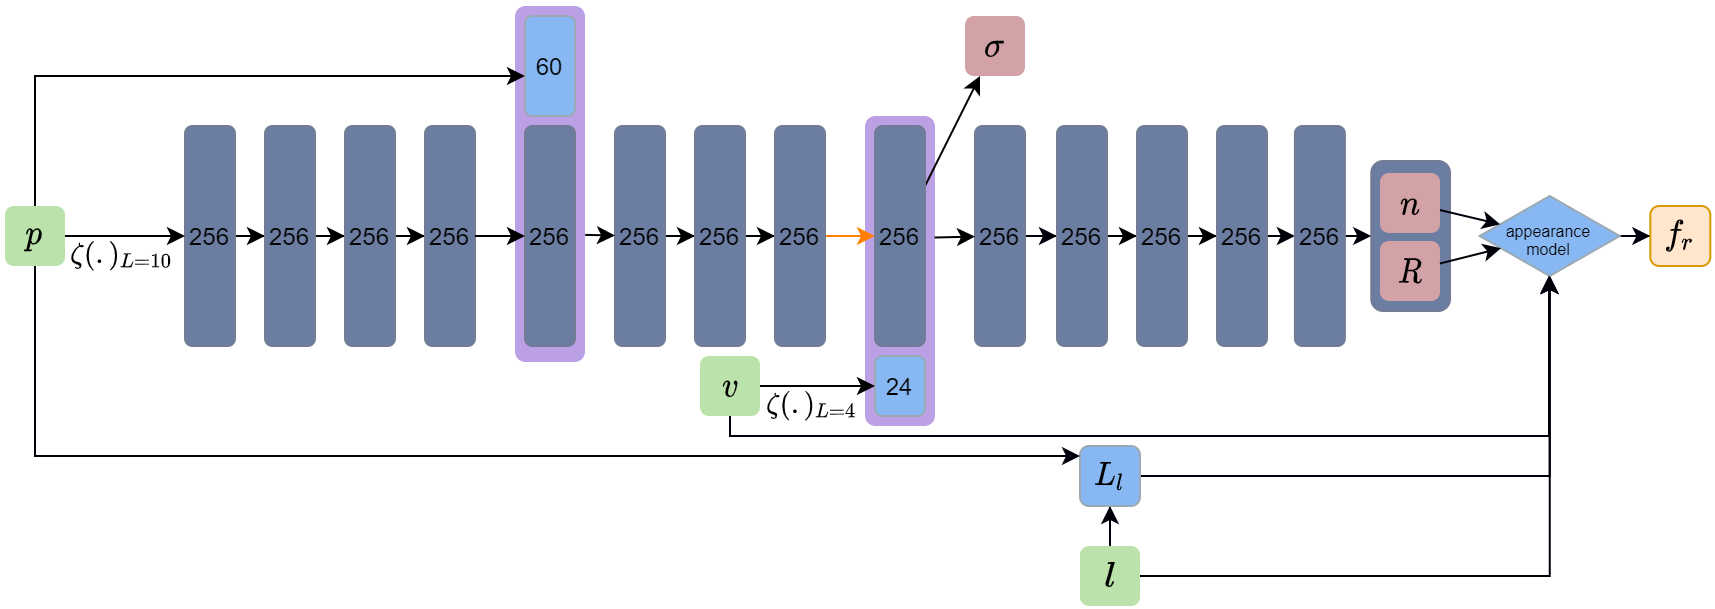
\includegraphics[width=0.9\textwidth]{figures/vanilla_nrf.png}
    \caption{MLP structure of the NRF \cite{bi2020neural} approach.
The overall network structure echoes the original NeRF model.
14 deep layers are used (instead of 10 in NeRF).
The appearance model block represents BRDF $f_r$
that is evaluated for each sample point $p$.
To this end network outputs normal $n \in \mathbb{R}^3$
and BRDF parameters $R \in \mathbb{R}^m$ ($m=4$ for microfacet BRDF).
$L_l$ denotes light intensity with consideration to distance attenuation.
}
    \label{fig:nrf_structure}
\end{figure}

The architecture of the MLP is outlined in \Cref{fig:nrf_structure}.
The deeper structure is used as the model capacity has to be increased
due to higher complexity of the task.
For each view sample point $p$ model outputs both normal vector $n$ and parameters $R$,
which are required by the selected BRDF model.
For the microfacet BRDF (\cite{walter2007microfacet}) $R$ consists of 3-dimensional albedo value
and 1-dimensional roughness value.



This formulation covers the general case when light source can be located at arbitrary position ('arbitrary setting').
Since the $l$ and $v$ vectors are different,
the additional sampling of light ray for each view sample point is required.
It makes this problem impractical. %infeasible.
However, \cite{bi2020neural} show that one specific light setting exist,
which can be used to handle this problem.
When the light ray $l$ coincide with the view ray $v$,
then sampling points $p(z)$ and $p'(z)$ would be the same,
which in turn means that $\tau_c(p_i) = \tau_l(p_i)$ ('co-located setting').
In this case there is no need in additionally sampling light rays,
which leave the processing time requirements on the same level as original work by \cite{mildenhall2020nerf}.
% \Cref{fig:colocated_light_source} \im{add figure} shows this process in more details.
Another advantage of this setting is that it has an accessible real-world analogy.
In particular, all of modern cellphones are equipped with cameras
and flash lights that are placed close to each other.
On the scale of the scene this displacement can be neglected and the setting can be considered to be co-located.

The co-located setting results in a very sparse sampling of the scene in terms of light-view directions.
During training there are no other samples
where angle between light and view rays is greater than zero.
This fact negatively affects the overall training performance,
although \cite{bi2020neural} claim
%proves
that even with these restrictions
the network is still able to generalize and reconstruct the scene appearance in high quality.
Authors also show some renders where the 'arbitrary setting' had been used during prediction phase.





\section{Explicit Neural Reflectance Field}
\label{sec:explicit_scheme}

The described above methods have already achieved some appealing results.
However, all of them have their own limitations that in either event reduce the performance either qualitatively (no light interaction) or quantitatively (too slow).
The explained below solution is constructed to take advantages from both NRF and NSVF approaches.
This method is later referred as 'brute-force scheme' as it performs the light rays sampling without any approximation techniques.

Since the NRF approach \cite{bi2020neural} is based on NeRF, it inherits its poor performance behaviour
and forces it to be only applicable for the 'co-located setting'.
Although the authors are even able to render the scene within 'arbitrary setting'
when only being trained on the co-located dataset,
the sparsity of the training dataset still highly affects network's generalization opportunities.

\cite{liu2021neural} in turn propose the technique for increasing the effectiveness of the training
for the color-based original NeRF approach.
The usage of gradually refined octrees gives more control over the sampling process
and makes the whole training phase faster.

\begin{figure}[!htb]
    \centering
    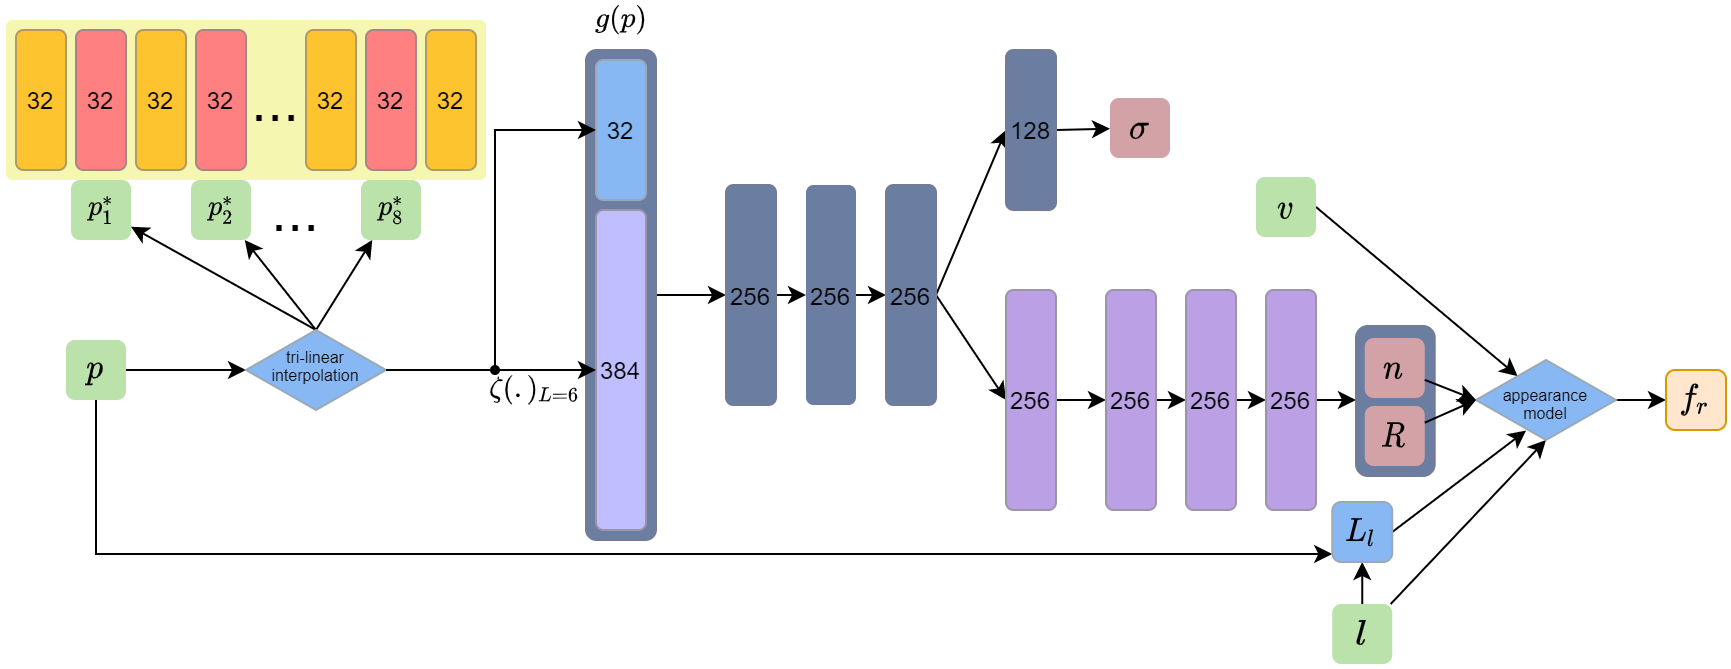
\includegraphics[width=0.9\textwidth]{figures/explicit_scheme.png}
    \caption{Model architecture for the 'explicit scheme'
    (\Cref{sec:explicit_scheme}).
The overall structure follows one from NSVF work.
The outputs of the network are similar to the NRF model.
BRDF evaluation ('appearance model' block) is required for achieving $f_r$ value.
    }
    \label{fig:mlnrf_bfex}
\end{figure}

Since both works NSVF and NRF use original NeRF framework,
in particular similar numerical integral estimation,
the process of reformulating NSVF problem to work with light radiances instead of color values is fairly straight forward.
For the integral estimation \Cref{eq:integral_estimation} is directly replaced with \Cref{eq:integral_estimation_nrf}.
The network architecture follows the guidelines from the NSVF work,
namely the encoder is shallow while texture predictor is deeper
comparing to the original NeRF method.
Appearance model block (right blue rhombus) includes BRDF evaluation,
which results in $f_r$ value required for final radiance calculation (using integral estimation formula \cref{eq:integral_estimation_nrf})

In order to train model on arbitrary light dataset
an additional step of light rays sampling and volume density prediction is needed.
This requires some nested model evaluations in order to retrieve $\sigma$ values at light sample points.
This is a quite memory intense part, however the lower model size comparing to the NRF approach makes it more accessible.
Another key note here is that there is no need in getting texture field predictions,
as for light rays the only valuable information is the volume density.
This allows to only evaluate the corresponding part of model.

Another key point here is the format of the dataset.
The NeRF and NSVF methods only work with color values,
which allows them to use the LDR images in the datasets
(i.e. PNG, JPG image formats and others).
However, NRF approach imply light intensity values that are integrated in final radiance calculations.
The LDR images are usually lacking the information of radiances
and only operate with color values.
All these facts make the LDR images bad candidates for the training dataset.
One should instead consider using HDR images (i.e. HDR, EXR formats).

The point light intensity value $I$ that takes part in calculation of $L_l(p, l) = f_{att} \cdot I$
represents the radiation power of the light source.
This value is known when processing artificially generated scenes
and thus can directly be used as value of $I$.
The real-world scenes (e.g. captured with the cellphone and flash light)
on the contrary does not have the exact light intensity value.
One could estimate the power of the flash light, but this would give only a rough estimation.
To make the method robust to this kind of estimations,
the light intensity value $I$ is passed to optimizer (along with other model parameter $\Theta$).
This technique requires some robust estimation of $I$ as an initialization value as well as an increased learning rate.



\section{In-Voxel Light Approximation}
\label{sec:invoxel}

Using sparse octree voxels for increasing the efficiency of the method
makes the whole problem feasible within some commonly accessible hardware.
However, the training procedure still remained highly computationally expensive and memory demanding
and therefore very slow in training or still even intractable for high resolution scenes.

The main load of this approach still remains in the additional sampling of light rays
and the consecutive model evaluation for calculating $\tau_l(p', l)$.
This fact leads to the task of minimizing the overhead that is caused by calculating light ray transmittances.

Predictions of volume densities at view ray sample points have primary importance
as they contribute into the final radiance value the most.
This assumption brings to the fact that light rays are not required
to be sampled as densely as view rays to remain the same level of accuracy.
Thus the lower number of points can be sampled on the light rays,
which would result in lower memory and time consumption.
However, this approach only alleviates the problem while not solving its route cause.

The octree structure that is used to encode feature vectors $\Tilde{g_i}$ in the corners of voxels
represent itself a coarse geometry of the scene.
Starting with only a few voxels that cover the whole bounding box around the scene,
the voxels undergo the \textit{self-pruning} and \textit{refinement} procedure (explained in \Cref{subsec:pruning}),
which increase the detailing capabilities of the octree
by increasing the number of voxels, lowering its sizes and rejecting empty voxels.
After only a few steps of the aforementioned operations the overall voxel structure
repeats scene geometry with a considerable amount of accuracy.
These voxels that intersect with the light rays can be used as an estimation of volume densities.

% \begin{figure}
%     \begin{tabular}{ccc}
%           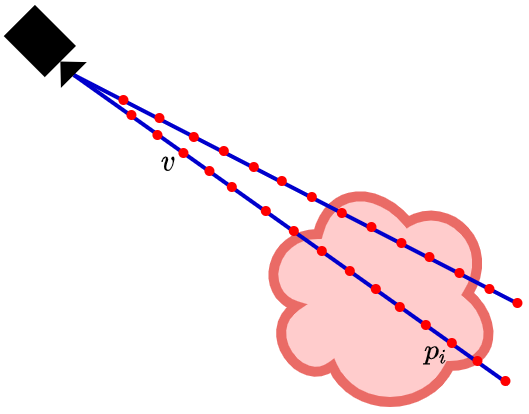
\includegraphics[width=0.1\textwidth]{figures/sampling_nerf.png}
%           & 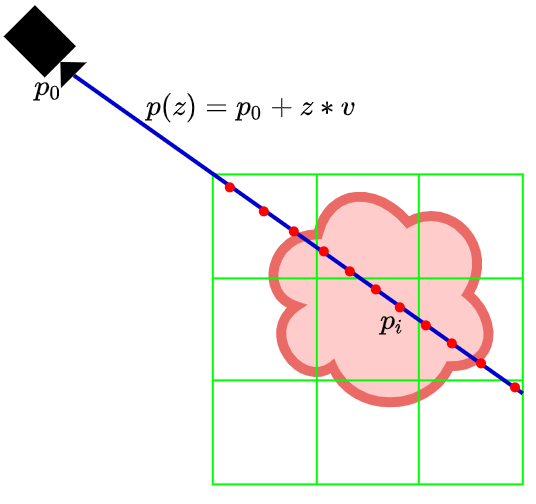
\includegraphics[width=0.1\textwidth]{figures/sampling_nsvf.png}
%           & 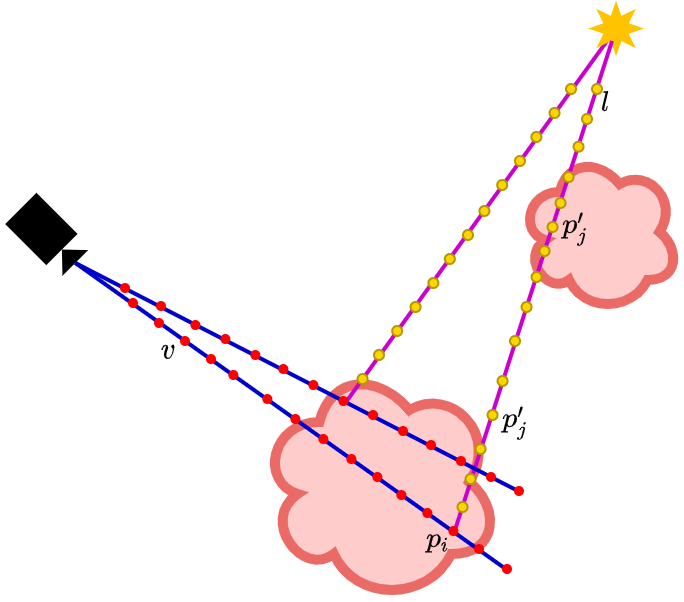
\includegraphics[width=0.1\textwidth]{figures/sampling_nrf.png}
%           \\(a) NeRF \cite{mildenhall2020nerf} & (b) NSVF \cite{liu2021neural} & (c) NRF \cite{bi2020neural}
%           \\[6pt]\multicolumn{3}{1}{
%               \begin{tabular}{cc}
%                 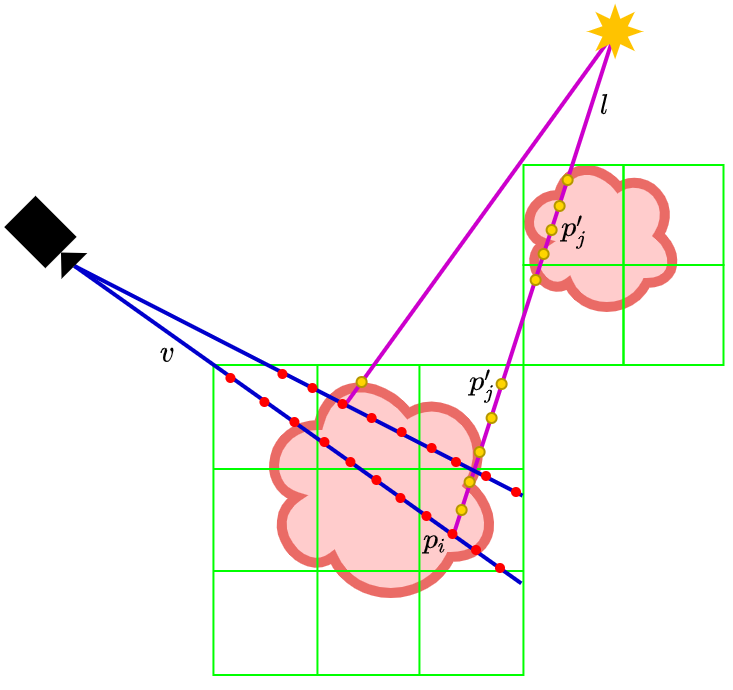
\includegraphics[width=0.1\textwidth]{figures/sampling_bfex.png}
%                 & 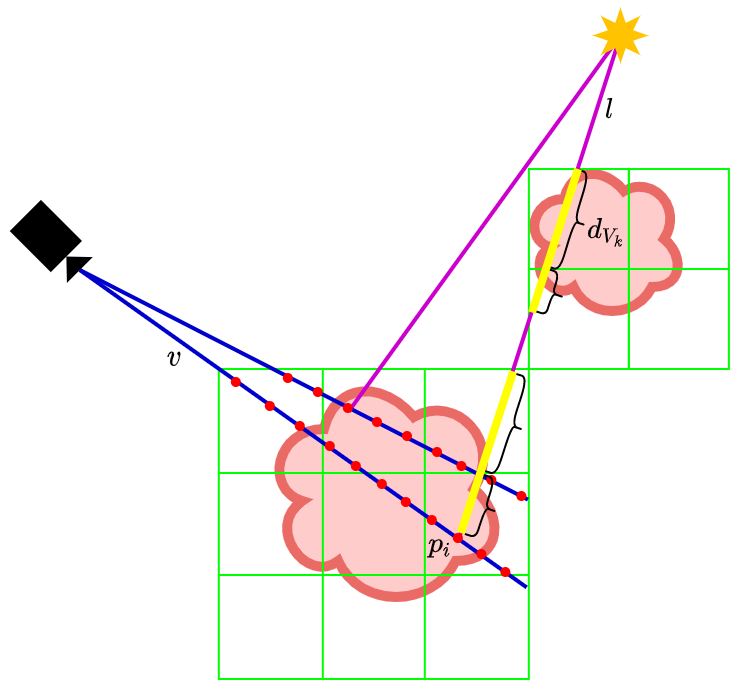
\includegraphics[width=0.1\textwidth]{figures/sampling_iva.png}
%                 \\[6pt](d) 'Brute-force' & (e) In-voxel approximation
%               \end{tabular}
%           }
%     \end{tabular}
%     \caption{caption}
% \end{figure}
\begin{figure}[!htbp]
    \begin{tabular}{ccc}
          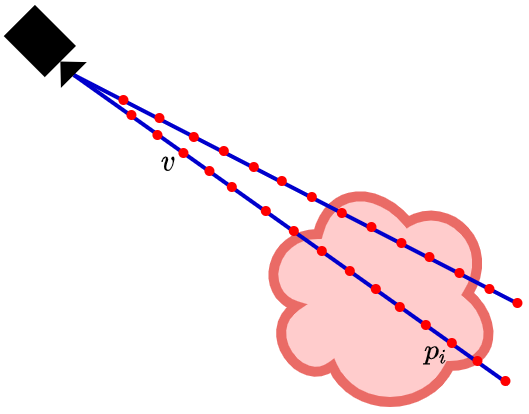
\includegraphics[width=0.285\textwidth]{figures/sampling_nerf.png}
          & 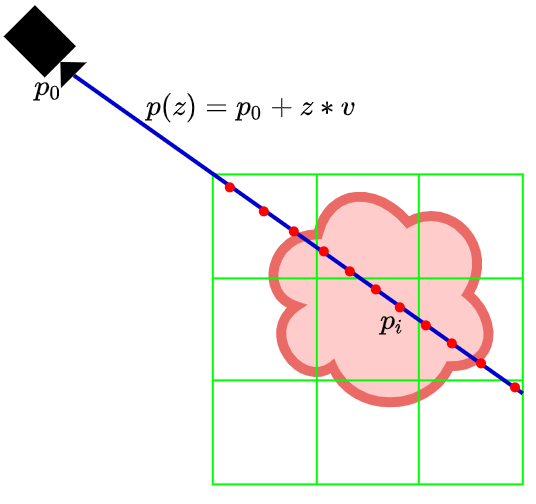
\includegraphics[width=0.26\textwidth]{figures/sampling_nsvf.png}
          & 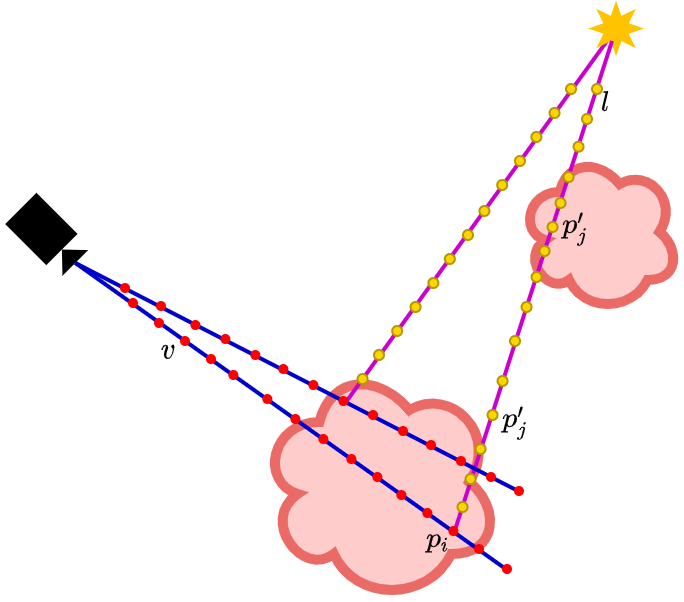
\includegraphics[width=0.355\textwidth]{figures/sampling_nrf.png}
          \\(a) NeRF \cite{mildenhall2020nerf} & (b) NSVF \cite{liu2021neural} & (c) NRF \cite{bi2020neural} (general)
          \\[6pt]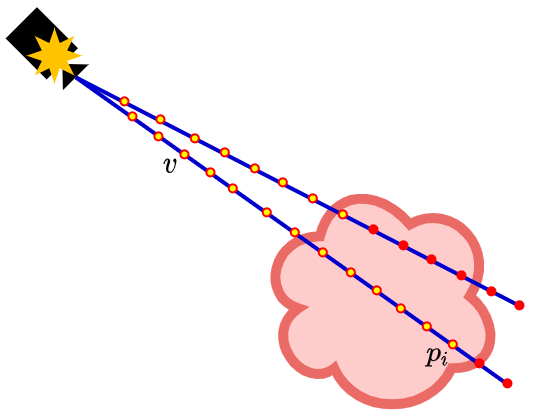
\includegraphics[width=0.26\textwidth]{figures/sampling_nrf_colocated.png}
          & 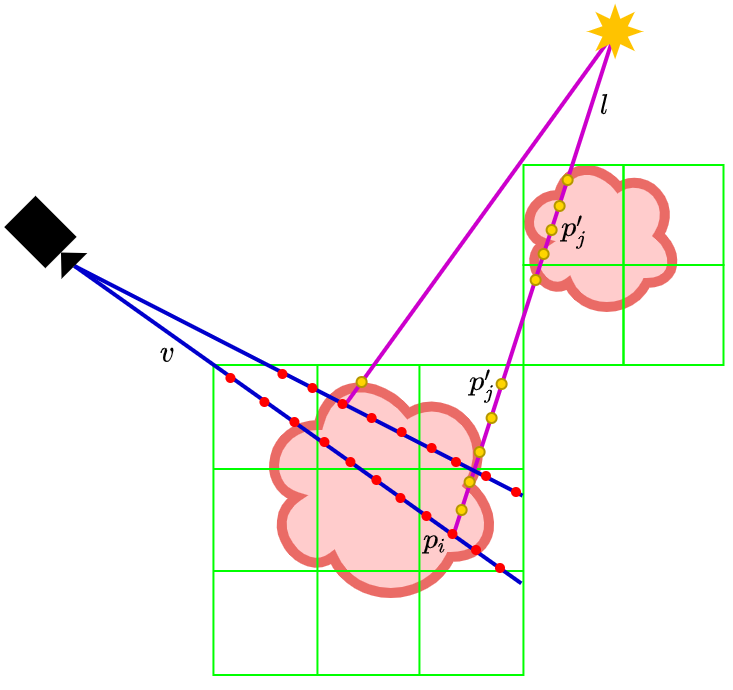
\includegraphics[width=0.32\textwidth]{figures/sampling_bfex.png}
          & 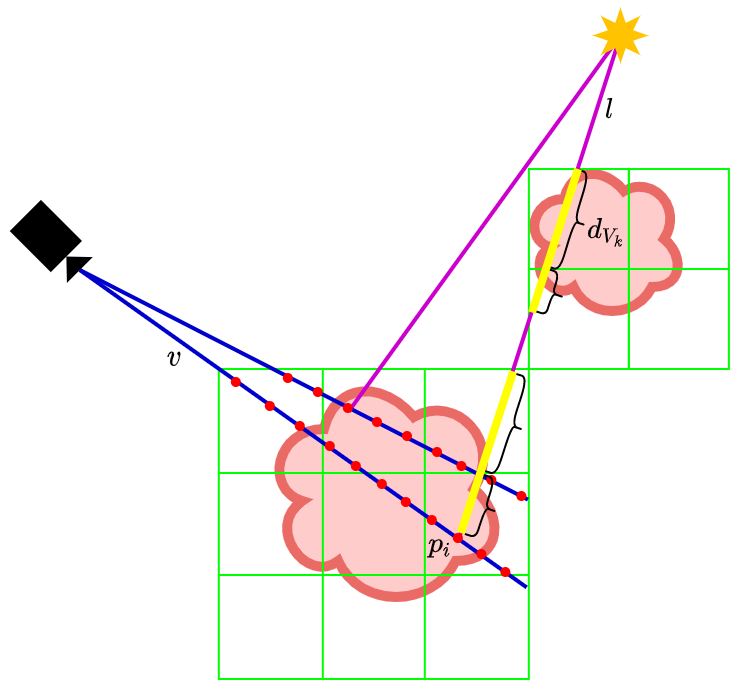
\includegraphics[width=0.32\textwidth]{figures/sampling_iva.png}
          \\(d) NRF (colocated) & (e) 'Brute force'& (f) In-voxel approximation
    \end{tabular}
    \caption{
Sampling techniques used in different approaches.
The 2D sketch schemes are used instead of 3D visualizations for simplicity.
Blue lines represent view rays $p(z)$ with direction vector $v$,
purple lines stand for light rays $p'(z)$ with light direction vector $l$
(only two of those are shown for brevity).
Red dots represent sampled view points $p_i$, yellow dots stand for light sample points $p'_i$.
Scheme (a) shows the original NeRF sampling technique without \textit{hierarchy sampling} (\Cref{subsec:hierarchy_sampling}).
Scheme (b) correspond to the NSVF sampling technique
that only occurs inside intersected voxels (represented by green boxes).
Scheme (c) shows sampling of the general case of the NRF approach
when light source is placed at arbitrary position.
Scheme (d) displays the 'colocated setting'
when point light source is positioned at the same location as camera.
In this case light sample points (yellow dots) coincide with the view sample points (red dots).
Scheme (e) correspond to the proposed in this work 'brute-force' approach
when light rays sampling is reduced by using the same voxel structure as in NSVF (fig. (b)).
Scheme (f) shows sampling proposed in this work in-voxel approximation scheme.
View rays are sampled equally as in NSVF approach
while light ray transmittances are estimated using travelled distances $d_{V_i}$
of the light ray inside voxels.
}
\label{fig:samplings}
\end{figure}

There are plenty of techniques that can be applied here in order to calculate light transmittances more efficiently.
The main proposed technique imply the assumption
that the volume density is homogeneously distributed inside the voxel.
This assumption is certainly wrong for general case,
but should give a fair estimation for the light ray transmittances.
In this case the travelled distance $d_{V_k}$ of the ray inside voxel $V_k$
can be used to weigh some value $\hat{\sigma_{V_k}}$ (\Cref{fig:samplings} f):
\begin{equation}
    \label{eq:light_ray_transmittance}
    \tau_l(p_i, l) = \exp \sum_{V_k \in \mathbb{V}^*} -\hat{\sigma}_{V_k} \cdot d_{V_k},
\end{equation}
where $\tau_l(p_i, l)$ is the light transmittance value at the view sample point $p_i$
and $\mathbb{V}^* \subset \mathbb{V}$ is the set of voxels $V_k$
that have been intersected by the light ray $p'(z') = p'_0 + z' \cdot l$.

The model can be periodically evaluated to predict the values of $\hat{\sigma}_{V_k}$ and consequently calculate $\tau_l$.
The period of evaluation can be similar to periods for \textit{self-pruning} and \textit{refinement} procedures
as some coarse value would already give an acceptable level of certainty.

Some other options can be applied here such as:
\begin{enumerate}
    \item calculate $\hat{\sigma}_{V_k}$ using points sampled in centers of voxels $V_k \in \mathbb{V}^*$
    \item calculate mean $\hat{\sigma}_{V_k}$ value from points of intersection of light ray with voxels $V_k \in \mathbb{V}^*$ (requires handling of edge cases)
    \item assign $\hat{\sigma}_{V_k} = \const, \forall V_k \in \mathbb{V}^*$
    \item use $\hat{\sigma}_{V_k}$ that was calculated during pruning stage
\end{enumerate}



\section{Implicit Neural Reflectance Field}
\label{sec:implicit_scheme}

The aforementioned methods that are proposed within this work
extend existing approaches in terms of efficiency for the problem of reproducing the scene under novel view and light conditions.
The novel light conditions is the essential requirement here
as it expects the method to not only account for color values
but also care about the reflectance of the surface.
Although, the NRF approach is formulated in general form
when any differentiable appearance model can be used for final radiance evaluation,
the result is still limited by the chosen BRDF.

\begin{figure}[!htb]
    \centering
    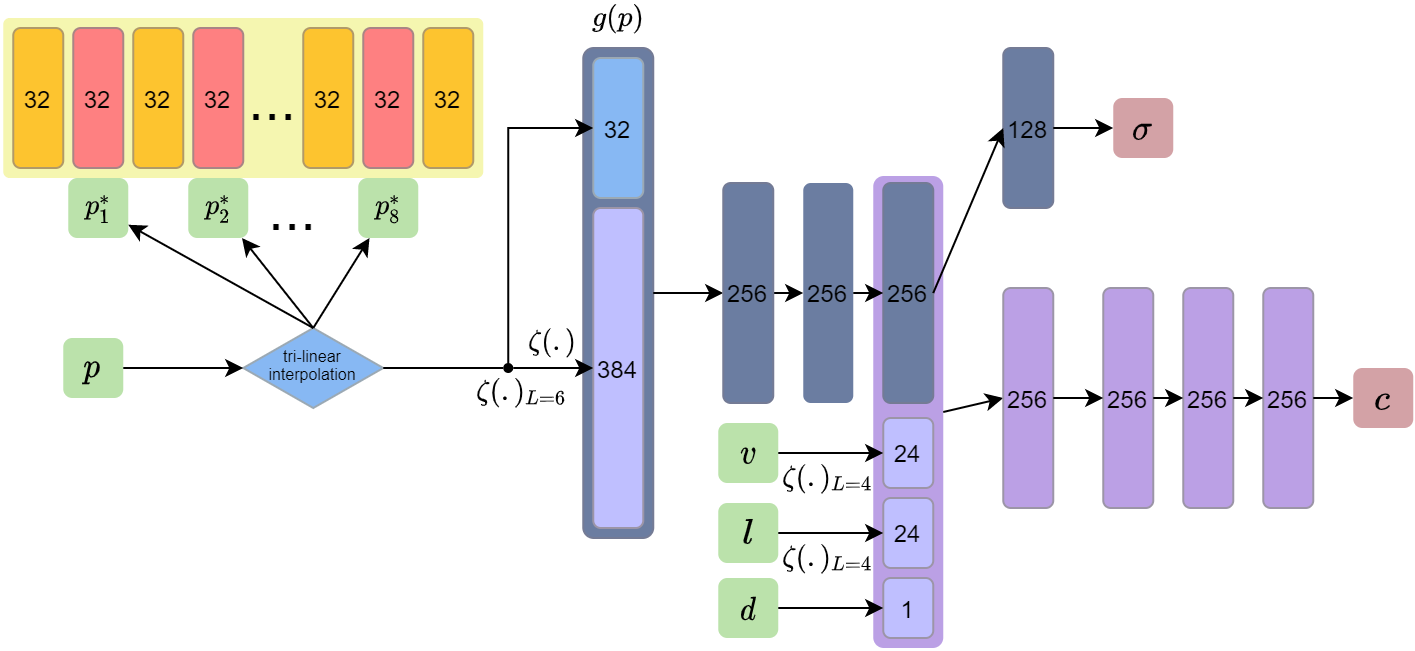
\includegraphics[width=0.9\textwidth]{figures/implicit_scheme.png}
    \caption{Network architecture for the implicit scheme.
The structure of the network mostly remains the same as in original NSVF work.
Some additional parameters such as light ray direction $l$
and distance $d$ from view sample point $p$ to the point light
are provided in advance into texture predictor.
}
    \label{fig:implicit_scheme}
\end{figure}

To avoid
%expand
these limitations one can shift the appearance evaluation burden to the deep neural network,
which is able to get trained for a very complex appearance representations.
This 'implicit scheme' would have a simpler neural network structure,
which is shown on \Cref{fig:implicit_scheme}.
The light interaction is performed here implicitly by providing 
the network the light direction $l$ as well as distance from sample point to the light source $d_i = \norm{p^l_k - p_i}$
as denoted on figure.
Light ray direction $l$ is also positionally encoded with the same $L$ as view ray direction $v$ is.

Another property of this technique will be the increased complexity of the learning function,
which would expect the network structure with greater capacity.

\im{\textit{Disadvantage: almost no control over implicit representation}}



% \section{Implicit Neural Reflectance Field}

% Existing BRDF models limits the type of scenes that can be captured
% and successfully reconstructed afterwards.
% To model object appearance one can employ neural network, which is able to get trained for a very complex appearance representations.
% In this work I \im{we?} call this technique as "Implicit scheme".

% Texture predictor not only is dependant on view direction,
% but also requires the light direction and distance to light source
% (for modelling the light attenuation effect).
% Figure \# shows the network structure for this approach.

% \begin{enumerate}
%     \item Light rays are not sampled (-> varying light transmittance either not considered or assumed to get learned by network\im{???})
%     \item |--> Tangential space for coordinates (and parametrization as half-vectors. not done)
% \end{enumerate}

% Since the appearance effects happen mostly in a local coordinate frame, the usage of the global direction vectors implies on the model to learn global to local coordinate system transformation. Although this is generally achievable, the overall complexity of the task can be too overwhelming for the model and some kind of correlations might affect the model. In order to increase the training performance this transformation can be done deterministically and the view and light directions in local coordinate frame are to be passed to the input of the model.

% The usage of the cartesian vectors is not very effective for reflectance representations. The half diff vectors (rusinkiewicz parametrization) can be used instead of positionally encoded l and v.
% \sm{or in combination with positional encoding}

% \section{In-Voxel Approximation}

% Using the octree allows to approximate light rays sampling inside voxels in order to increase the performance of the method.

% Instead of performing inverse CDF sampling as it is done for view rays, one can do the following:
% \begin{enumerate}
%     \item Bravely \sm{colloquial} assume the media homogenious inside voxels and boldly approximate it as constant
%     \item Under the same brave assumption perform some sampling inside the voxel once at N iterations (e.g. right after pruning has been performed)
%     \item The in-voxel sampling can be lighter than inverse CDF (e.g. just sample the center of voxel, or voxel corners + trilinear interpolation)
% \end{enumerate}







% NSVF proposed a good technique of using Sparse Voxel Trees in order to increase the rendering speed. However, the scene is still lacking the light interaction.

% One can achieve this by also passing light directions along with distance to the light source into the network, in order to make it distinguish different surface properties for different view and light directions.








% This is some test area for new mathematical helper macros to nicely visualize mathematical formulas.

% \section{Numbers}
% \begin{align}
%     \mathbb{C}
%     \qquad
%     \mathbb{R}
%     \qquad
%     \mathbb{Q}
%     \qquad
%     \mathbb{Z}
%     \qquad
%     \mathbb{N}
% \end{align}

% \section{Numbers with physical units}
% \begin{align}
%     \SI{1.23}{\meter\per\second}
% \end{align}
% \begin{align}
%     \si{\meter\per\second}
% \end{align}
% \begin{align}
%     \SI{1.23\pm0.45}{\meter\per\second}
% \end{align}
% \begin{align}
%     \SI{3e8}{\meter\per\second}
% \end{align}
% \begin{align}
%     \SI{32}{\giga\byte} = \SI{32e9}{\byte}
% \end{align}
% \begin{align}
%     \SI{32}{\gibi\byte} = \SI[exponent-base=2]{32e30}{\byte}
% \end{align}

% \section{Norm, Dot, Abs, Interval}
% \begin{align}
%     \pi = \const
% \end{align}
% \begin{align}
%     1 \in \interval{0}{2}
% \end{align}
% \begin{align}
%     1 \in \order{n}
% \end{align}
% \begin{align}
%     \evalat{ \frac{\partial f}{\partial x} }{ x = 0 }
% \end{align}
% \begin{align}
%     \norm{p} \qquad \norm{\frac{p}{2}}
% \end{align}
% \begin{align}
%     \abs{p} \qquad \abs{\frac{p}{2}}
% \end{align}
% \begin{align}
%     \dotproduct{p}{q} \qquad \dotproduct{\frac{p}{2}}{q}
% \end{align}
% \begin{align}
%     \crossproduct{p}{q} \qquad \crossproduct{\frac{p}{2}}{q}
% \end{align}

% \section{Vector, Matrix}
% \begin{align}
%     \vec{p} \qquad \vecarrow{p}
% \end{align}
% \begin{align}
%     \vec{p}^{\transposed}
% \end{align}
% \begin{align}
%     \gradient{\vec{p}}
% \end{align}
% \begin{align}
%     \divergence{\mat{A}}
% \end{align}
% \begin{align}
%     \laplacian{\mat{A}}
% \end{align}
% \begin{align}
%     \mat{A}
% \end{align}
% \begin{align}
%     \set{K} , K
%     \qquad
%     \set{N} , N
% \end{align}
% \begin{align}
%     \neighborhood{\vec{p}} = \left\{ \vec{q} \mid \norm{\vec{p} - \vec{q}} < \epsilon \right\}
% \end{align}

% \section{Set operations}
% \begin{align}
%     A \intersect B
% \end{align}
% \begin{align}
%     A \union B
% \end{align}
% \begin{align}
%     A \difference B
% \end{align}

% \section{Derivative, Integral, Sum, Probability}
% \begin{align}
%     \int_H x \, dx
% \end{align}
% \begin{align}
%     \sum_H x
% \end{align}
% \begin{align}
%     \probability{x}
% \end{align}
% \begin{align}
%     \probabilitygiven{x}{y}
% \end{align}
% \begin{align}
%     \expectation{x}
% \end{align}
% \begin{align}
%     \deviation{x}
% \end{align}
% \begin{align}
%     \variance{x}
% \end{align}


% \section{Lemma, Theorem, Corollary}
% \begin{lemma}
%     This is a lemma.
% \end{lemma}
% \begin{proof}
%     Proof of lemma.
% \end{proof}

% \begin{theorem}
%     This is a theorem.
% \end{theorem}
% \begin{proof}
%     Proof of theorem.
% \end{proof}

% \begin{corollary}
%     This is a corollary.
% \end{corollary}
% \begin{proof}
%     Proof of corollary.
% \end{proof}


